%***********************
\chapter{Introducción}
\label{cap.introduccion}
\pagenumbering{arabic} 
%***********************

Las primeras truchas en Chile hacen su aparición a fines del siglo XIX, específicamente en 1880, fue en este año cuando en la recién hace 5 años fundada ciudad Lota, actual región del Bio-Bio se introdujeron las primeras ovas de la llamada “Trucha común”, actualmente conocida como Trucha Fario (*Salmo trutta*). No fue hasta en la primera década del siglo XX que el gobierno de ésa época, respondiendo a las inquietudes de un naturalista alemán llamado Federíco Albert, quien había realizado un catastro de las posibles especies de salmónidos que podrían ser introducidos en nuestro país, el cual reconoce el potencial poder económico de estos salmónidos e introduce, junto a la creación de la Piscicultura Río Blanco, tres especies traídas desde Francia, la Trucha Fario, la Trucha arcoíris (*Oncorhynchus mykiss*) y el Salmón del atlántico (*Salmo salar*).
\section{El género \emph{Oncorhynchus}}
Onchorhyncus corresponde a uno de los 10 generos de la familia Salmonidae y tiene alrededor de 12 especies, incluyendo *O.mykiss* (trucha arcoíris), *O. nerka* (salmón rojo), *O. gorbuscha* (salmón rosado), *O. tshawytscha* (salmón chinook), *O. kisutch* (salmón coho) , entre otros. Se distribuyen principal y naturalmente por una vasta zona que comprende desde California hasta el mar de Behring y el oceáno ártico [@groot1991pacific].

Algunas características principales de este genero son las siguientes

- Son peces anádromos, es decir emigran al mar cuando son juveniles y luego vuelven al agua dulce para reproducirse.
- A su vez, en su mayoria solo se reproducen una vez, por lo tanto son semélparos.
- Tienen baja tasa de fecundidad (2 a 5mil ovas) y grandes huevos (5-8mm)

En Chile encontramos la Trucha arcoíris, el Salmón coho (*Oncorhynchus kisutch*) y el Salmón chinook (*Oncorhynchus tshawytscha*) como representantes de este genero.

La trucha arcoiris, descrita inicialmente por Walbaum en 1972 tiene un cuerpo alargado fusiforme con 60 a 66 vertebras, con 3 a 4 espinas dorsales, 10 a 12 rayos dorsales blandos, 3 a 4 espinas anales, 8 a 12 rayos anales blandos y 19 rayos caudales. Presentan una aleta con gran tejido adiposo, la cual usualmente contiene un borde negro. Tienen como coloración principal tonalidades de azul a verde oliva, sobre una banda rosa a lo largo de la linea lateral y plateada por debajo de ella, configuración cromática que le da su nombre *arcoíris*.

\begin{figure}[h!]
	\centering
	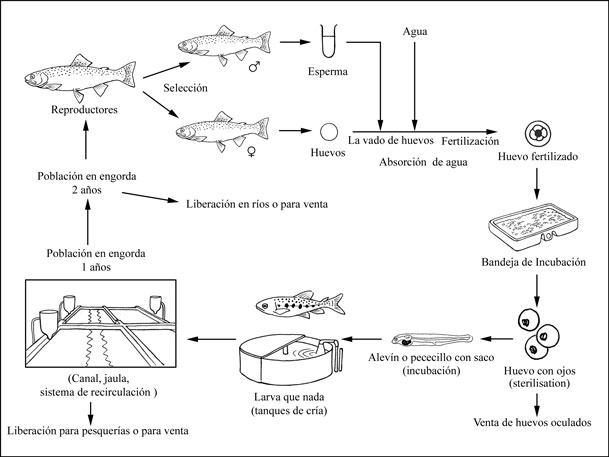
\includegraphics[width=11cm]{1} 
	\caption {Ciclo productivo de la trucha arcoíris}
	\label {fig:ciclo}
\end{figure}

Este pez es resistente, de crecimiento rápido y tolerante a una amplia gama de manipulaciones y ambientes, pudiendo así ocupar una variedad de hábitats y diferentes temperaturas. La temperatura ideal para el cultivo de la trucha arcoíris está por debajo de 21º C, aunque en etapa de desove y crecimiento la temperatura tiene que estar en el rango de 9 a 14ºC (Figura \ref{fig:ciclo}).

\subsection{Situación actual en Chile}

Los desembarques de Trucha arcoíris han aumentado cercano al 1500\% en 20 años (Figura \ref{desembarques}), con una tasa de crecimiento porcentual promedio del alrededor del 15\% [@sernapesca2012], en términos monetarios, el año 2013 la exportación de este producto genero ventas alrededor de los 300 millones de dólares, lo que lo convierte en una de las 3 especies más cosechadas en Chile junto al Chorito y el Salmón del atlántico [@subpesca2013].

\begin{figure}[h]
\begin{tikzpicture}
\begin{axis}[
axis lines*=left,
ybar,
scaled y ticks=false,
ylabel={Toneladas},
xlabel={Año},
xlabel absolute, xlabel style={yshift=-0.5cm},
ylabel absolute, ylabel style={yshift=0.5cm},
xtick={1992, 1993, 1994, ..., 2012},
  /pgf/number format/.cd,
        use comma,
        1000 sep={},
x tick label style={rotate=45,anchor=east},
yticklabel style={/pgf/number format/fixed},
width=14cm, height=7cm]
\pgfplotstableread[col sep=comma, header=has colnames]{datos/desembarques.csv}\loadedtable;

\addplot table[x=Año, y=Toneladas] {\loadedtable};
\end{axis}
\end{tikzpicture}
\caption{Desembarques de Trucha arcoíris en Chile} \label{desembarques}
\end{figure}

Uno de los principales aspectos a tener en cuenta con una especie con tal valor comercial es su respuesta inmune. Gran parte de la mortalidad de estas especies deriva de distintos tipos de infecciones, como por ejemplo las provocadas por *Flavobacterium psychrophilum* y *Piscirickettsia salmonis*, llegando a haber muertes en casos de hasta el 50\% y 34\% de la producción respectivamente. La explicación de esto radica en la pérdida del equilibrio ambiente-patógeno-hospedero, lo cual genera las condiciones que hacen aumentar la enfermedad y mortalidad en el cultivo. En el caso de la acuicultura (Industria que representa cerca de un 50\% de la oferta mundial de pescado) [@FAO2012], un grave problema son las enfermedades asociadas a cultivos masivos de peces, mayoritariamente relacionadas al stress en que se ven sometidos los organismos como también por el crecimiento acelerado de la producción y los sistemas de cultivo actuales [@FAO2012; @Georgiadis2001]⁠⁠. Estas enfermedades, cualquiera sea su origen, pueden tener un alto impacto negativo en la producción mundial, lo que equivale a grandes pérdidas económicas [@Shao2001]⁠. Por lo tanto es necesario tener información del sistema inmune en peces, para así poder minimizar los efectos producidos por estas enfermedades y en algunos casos prevenirlos.


\section{Sistema inmune en peces}
La comprensión de la funcionalidad del sistema inmune de peces, especialmente en teleósteos, al igual que en vertebrados superiores se puede entender como una respuesta innata o inespecífica y una respuesta adaptativa o especifica. La respuesta inmunológica presentada por los peces está bien desarrollada e integrada, aunque si, influenciada notoriamente por los cambios estacionales y la temperatura [@Fernandez2002; @Olabuenaga2000]

La respuesta inmune innata o inespecífica en peces es muy importante, ya que constituye la primera y más importante línea de defensa del pez frente a un gran número de patógenos, en esta respuesta convergen factores humorales y celulares [@Fernandez2002; @Olabuenaga2000; @Zhu2012]. Este tipo de inmunidad está basado en el reconocimiento no clonal de los componentes estructurales o secretados de los patógenos microbianos [@Athman2004]⁠, los cuales son llamados patrones moleculares asociados a patógenos (o PAMPs, por sus siglas en inglés), estos a su vez son reconocidos por receptores de reconocimiento de patrón (PRR, por sus siglas en inglés) [@Gordon2002], entre los cuales se encuentran receptores de tipo Toll (TLR, por sus siglas en inglés), el receptor de complemento tipo-3 (CR3), Dectina-1, proteína C-reactiva, entre otros [@Rondon-Barragan2010]. Entre los PAMPs más clásicos se puede encontrar a las secuencias de ADN CpG sin metilar, los lipopolisacáridos (LPS) y el RNA bicatenario viral. La interacción entre los PRR (como los TLR) y los PAMP es la reacción que desencadenará e iniciará la transducción de señales intracelular que resultara en la expresión de genes involucrados en la inflamación, respuesta antiviral y maduración de células con fenotipo dendrítico [@Aghaallaei2010]⁠; TLRs individuales activan factores de transcripción únicos y comunes a través de diferentes vías de señalización para generar una respuesta biológica especifica ante microorganismos [@Bols2001; @Ellis2001; @Kawai2005]

Entre las células involucradas la fase celular inespecífica de la respuesta inmune están las células citotóxicas no específicas (NCC, por sus siglas en inglés), células fagocíticas, y granulocitos [@Ainsworth1992; @Ellis1977]. Las células NCC en peces se encuentran principalmente en el riñón cefálico, el bazo, sangre periférica y el timo, son células citotóxicas inespecíficas, es decir ejercen su acción en diferentes células diana sin un reconocimiento previo, las cuales requieren un contacto célula-célula para poder efectuar la lisis celular [@Graves1984]. Dentro de las células fagocíticas los neutrófilos representan aproximadamente en promedio a un 11\% de los leucocitos en sangre, son también llamados polimorfonucleares o leucocitos específicos, su capacidad fagocítica es baja, ya que ingieren poco material extraño, aunque poseen la mayoría de la batería enzimática para este trabajo. Los eosinófilos y basófilos son los granulocitos con menor presencia en peces, aunque en el caso de los eosinófilos se han logrado encontrar en peritoneo u otros tejidos como el intestino, mientras que los basófilos tienen escasa presencia en estos organismos [@Palic2011].

Dentro del sistema fagocítico mononuclear, podemos encontrar a los monocitos y a los macrófagos (derivados de estas últimas), los primeros son móviles y generalmente más grandes que los demás leucocitos, en el caso de los macrófagos, pueden fagocitar partículas mucho más grandes, son abundantes en el bazo y riñón cefálico, aunque también se han encontrado en mucosa olfatoria [@Castro2011; @Olabuenaga2000].

Entre los componentes moleculares asociados a la respuesta innata del sistema inmune de peces podemos encontrar a las citoquinas, las cuales son una familia de proteínas de bajo peso molecular (comúnmente glicosiladas) y secretadas por células del sistema inmune activadas previamente frente a la exposición de diferentes componentes patógenos [@Salazar-Mather2006]⁠. Estas citoquinas pueden dividirse en interferones (IFNs), interleuquinas (ILs), factores de necrosis tumorales (TNFs, por sus siglas en inglés), factores estimuladores de colonias y quimioquinas [@Savan2006]⁠. Las interleuquinas son citoquinas producidas principalmente por linfocitos T CD4+, aunque también son secretadas por una gran variedad de tipos celulares, como por ejemplo los macrófagos/monocitos y las células endoteliales [@Secombes2011b], las quimioquinas, o también llamadas citoquinas quimiotácticas (o quimioatractantes) son una familia de citoquinas que son liberadas por la mayoría de tejidos infectados en los estadíos tempranos de infección. Las citoquinas pueden dividirse en distintas familias según sea la organización de sus cisteínas. 

Dentro de la familia de las interleuquinas podemos encontrar la Interleuquina 1$\beta$, la citoquina proinflamatoria mas estudiada, todo debido a su rol mediador de enfermedades autoinflamatorias. Es producida principalmente por macrófagos activados, celulas dendríticas y monocitos, y afecta a casi cualquier tipo celular, jugando un rol central en la generación de respuestas sistémicas y locales a la infección, asi como también en respuesta a daños y desafíos inmunológicos [@Reis2012]. Esta citoquina potencialmente induce la proliferación, diferenciación y activación de celulas no específicas, como NK, macrofagos, etc..., así como también una respuesta inmune específica, activando linfocitos B y T  [@Taechavasonyoo2013; @Hong2004]. Junto con IL-1$\beta$ existe otro marcador que sirve para evaluar si es que los inmunoestimulantes inducen o no una respuesta inflamatoria, este otro marcador es el Factor de necrosis tumoral (TNF$\alpha$). este factor tiene una variedad de funciones inmunológicas, regulando la inflamación y la respuesta inmune celular[@Zou2003; @Teles2011; @Wang2004]. Promueve la necrósis hemorrágica de tumores, así como también mejora la fagocitosis y citotoxicidad de neutrofilos. Mejora la sintesis de prostaglandina E2 y oxido nítrico (NO), y modula la expresión de muchas citoquinas, incluyendo IL-1, IL-6 y algunas quimioquinas. IL-1$\beta$ y TNF$\alpha$ son ampliamente usados como marcadores de respuesta inmune innata [@Zhang2009].

Otra citoquina importante en el proceso inmunitario es Interferón Gamma (IFN$\gamma$), perteneciente a la familia de los Interferones, moleculas encargadas principalmente en la respuesta viral, aunque también son importantes reguladores del sistema inmunitario innato y adaptativo [@Savan2006].  El IFN-$\gamma$ es producido en una primera etapa por celulas NK estimuladas por las interleuquinas 12 y 18, las cuales son producidas por fagocitos mononucleares y celulas presentadoras de antígenos (APCs, por sus siglas en inglés). Al ser secretada esta molécula se une a su receptor y por la via Jak/STAT promueve la activación de macrófagos aumentando la sintesis de la fagocito oxidasa dependiente de NADPH (\si{gp91^{phox}} y \si{p67^{phox}}), la oxido nítrico sintasa 2 (NOS2), p47 GTP-asa y la proteina de union a guanilato, así como también aumenta las moleculas de MHC de clase 2 en macrofagos y otras APCs [@Boehm1997]. Por lo tanto en contraste con los interferones de tipo I (IFN-$\alpha$/$\beta$) el IFN$\gamma$ juega un rol clave en la activación de macrofagos para aumentar destrucción de patógenos bacterianos, protozoos y virales [@fields2007fields].

La interleuquina 12 (IL-12) es una citoquina heterodimérica, compuesta por la subunidades P35 y P40, la primera miembro de la familia de la interleuquina 6 con 4 $\alpha$-helices en su topología y p40 recuerda una forma asociada a un receptor de citoquinas solubles[@Huising2006; @Yoshiura2003]. Esta citoquina pro-inflamatoria es producida en las etapas iniciales de la respuesta inmune por monocitos, macrófagos, celulas dendríticas y neutrofilos, y una de sus principales funciones es inducir la sintesis de otras citoquinas, como el anteriormente nombrado IFN-$\gamma$, que sirve como orquestador en la maduración de un linfocito T \emph{naive} a un fenotipo Th1 [@Nascimento2007], y es gracias a esta función se considera como un medidador entre la respuesta innata y adaptativa de la inmunidad [@Zhang2014].

Dentro de las moleculas efectoras de la respuesta inmune la oxido nítrico sintasa de tipo inducible (iNOS), propia de fagocitos [@Wu2008; @Zhao2010],  aumenta su expresión durante eventos de inflamación, y a su vez, es propia del estallido respiratorio de los macrófagos proveyendo así a la celula de un ambiente citotóxico ideal para los eventos pro-inflamatorios por la producción de Oxido Nítrico (NO), catalizando la oxídación de L-arginina [@Yang2013]. Esta molecula, puede ser activada en monocitos, macrófagos, células dendríticas, neutrofilos y células NK ya sea por citoquinas, endotoxinas, o ambas [@MacMicking1997; @Bogdan2001]. estas características demuestran  la importancia del rol de iNOS y su producto gaseoso NO en el sistema inmune, ya que a diferencia de las otras NOS, la neuronal (nNOS) y la endotelial (eNOS) esta no tiene una sintesis basal ni constitutiva, haciendo de esta molecula un marcador inmunológico de importancia para estudiar procesos inmunológicos.

Otras moléculas efectoras presentes en la respuesta innata frente a patógenos son los péptidos anti-microbianos (AMP, por sus siglas en inglés), moléculas con la capacidad de destruir y/o neutralizar microorganismos patógenos directamente, son moléculas pequeñas, anfipáticas y catiónicas [@Mercado2005]⁠, y están ampliamente extendidos por los reinos vegetal y animales [@Zasloff2002]. Los mecanismos de acción anti-bacteriana de estos AMP pueden entenderse desde dos puntos de vista diferentes: 1. La estructura anfipática puede unirse selectivamente a la membrana bacteriana y generar poros transmembrana, los cuales destruyen a la bacteria desintegrando la membrana, y 2, los AMP pueden directamente entrar a la bacteria e interactuar específicamente con factores de crecimiento y metabolismo bacteriano eventualmente generando la muerte bacteriana [@Wimley2010; @Zhu2012]⁠. Entre los péptidos anti microbianos descritos en peces podemos encontrar cuatro grandes grupos, las defensinas, proteínas de macrófagos asociadas a resistencia natural (Pramps, por sus siglas en inglés), NK-lisina y hepcidinas. 

Otra familia de péptidos antimicrobianos son las Catelicidinas, presentes generalmente en neutrófilos y superficies de mucosas, su actividad se centra principalmente en su interacción con la membrana plasmática de la bacteria para eventualmente destruirla, fueron primeramente descritas en mamíferos y luego se han encontrado en distintos peces teleósteos, algunos casos son los de trucha arcoíris [@Chang2005]⁠, bacalao [@Maier2008], salmón del atlántico [@Chang2006], entre otras.
Además de poseer una robusta y bien desarrollada respuesta inmune innata como se explicaba anteriormente, los peces también cuentan con una respuesta adaptativa, con componentes celulares y humorales [@Alvarez-Pellitero2008]⁠, en este último grupo se encuentran los anticuerpos, los cuales son proteínas pertenecientes al grupo de las inmunoglobulinas (Ig), en el caso de los peces producen inmunoglobulinas del tipo M, T y D [@Bengten2002; @Zhang2011; @Zhu2012]⁠, siendo la primera la más importante, estando presente en el suero, el mucus y la bilis. Los anticuerpos son producidos por linfocitos B activados al reconocer algún antígeno, ya sea en solución o presentado por alguna célula presentadora de antígeno, que en el caso de los peces principalmente son macrófagos, y tienen variadas funciones, pueden actuar como moléculas efectoras en el suero, o también como receptores de superficie de linfocitos B.

Una de las principales diferencias entre el sistema inmune de peces teleósteos con el de mamíferos es la carencia de medula ósea y ganglios linfáticos, por lo cual no se puede marcar una diferencia entre órganos hematopoyéticos y órganos linfoides [@Fernandez2002; @Olabuenaga2000]⁠. Entre los principales órganos pertenecientes al sistema inmune de peces podemos encontrar el timo, el riñón y el bazo. El riñón cefálico es el principal órgano en la diferenciación de linfocitos B, ya que es el primer órgano en el que aparecen estas células durante el desarrollo del pez, también es el órgano donde se produce la eritropoyesis, granulopoyesis, linfopoyesis y monocitopoyesis [@Whyte2007], por lo que se le puede considerar a la vez un órgano análogo a la medula ósea de los mamíferos [@Razquin1990]⁠. Los centros melanomacrofágicos son una agregación de macrófagos que contienen melanina, un pigmento de color oscuro, su tamaño y número está directamente relacionado con el estado del pez, ya que estas variables aumentan considerablemente en peces enfermos, donde el catabolismo ha sido excesivo. Algunos estudios ontogénicos realizados en salmónidos sugieren que la función del bazo no es esencial en la maduración del sistema inmunológico, ya que los linfocitos del timo y riñón cefálico estarían más involucrados que este órgano en esta maduración. Otros estudios sin embargo indican, que bajo un desafío antigénico aparecen linfocitos B en el bazo, teniendo parámetros similares a los presentados por estas células en otros órganos como el riñón cefálico.
\section{Inmunoestimulantes}

Los inmunoestimulantes han sido descritos como componentes necesarios para la acuicultura, ya que mejoran la respuesta innata y proveen resistencia a patógenos. Diferentes de estas sustancias, como los B-glucanos, productos bacterianos y constituyentes de las plantas pueden iniciar directamente la activación de mecanismos de defensa innata actuando en receptores y desencadenando la activación de distntos genes que puedan resultar en la producción de moleculas antimicrobianas [@Bricknell2005; @Kumari2006].
A pesar de la evidencia demostrada sobre el uso benéfico de estas sustancias como potenciales inmunomoduladores de la respuesta frente a disntitos patógenos en la acuicultura [@Abarca2012; @Bilen2011; @Bricknell2005; @Dalmo2008; @Chettri2013a], las actuales soluciones comerciales están de cierta manera restringidas por ser derivadas de algunas levaduras, como por ejemplo los B1-3,B1-6 glucanos que son vendidos bajo la marca MacroGard® y sus distintos derivados. Existe también un producto comercial llamado Ergosan, el cual está hecho de una mezcla de distintos componentes de un alga, la cual es rica en alginatos y polisacáridos. Una dosis individual de 1mg de Ergosan aumenta singificativamente la proporción de eutrofilos, aumentan el grado de fagocitosis, la actividad del estallido respiratorio y la expresión de interleukina 1B (IL-1B), interleukina 8 (IL-8) y el factor de necrosis tumoral alfa (TNF-$\alpha$) in leucocitos peritoniales de trucha arcoíris a 1 dia post inyección [@Peddie2002a].

\subsection{$\beta$-glucanos}

\begin{table}[h!]
	\sffamily
	\begin{center}
		\begin{threeparttable}
		\captionsetup{font={normalsize,sf}}
		\caption{Estructuras de $\beta$-Glucanos según su origen}\label{tablaglucanos}
			\begin{tabularx}{13cm}{l c X}
			\toprule
			\textbf{Origen} & \textbf{Estructura} & \textbf{Función} \\
			\midrule
			Bacteriano & 
\includegraphics[width=3cm]{bgbacteriano} & $\beta$1,3-Glucano lineal con ramificaciones largas de $\beta$1,6-Glucano\\
			Levadura & 
\includegraphics[width=3cm]{bglevadura} & $\beta$1,3-Glucano Lineal \\ 
			Cereal & 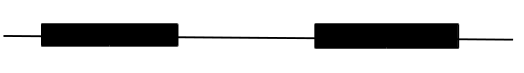
\includegraphics[width=3cm]{bgcereal} & $\beta$1,3/$\beta$1,4-Glucano lineal \\
			Hongo & 
\includegraphics[width=3cm]{bghongo} & $\beta$1,3-Glucano lineal con ramificaciones cortas de $\beta$1,6Glucano \\
			\bottomrule
			\end{tabularx}
			\begin{tablenotes}
			\item Estructuras de $\beta$-Glucanos según su origen
			\end{tablenotes}
		\end{threeparttable}
	\end{center}
\end{table}


Los $\beta$-glucanos son carbohidratos que consisten en moléculas de glucosas enlazadas, los cuales son componentes estructurales de gran importancia en paredes celulares de levaduras, hongos, algas y algunas bacterias. Estos carbohidratos también forman parte de la pared celular endospermas de algunos cereales como la cebada y la avena. Dependiendo del origen del $\beta$-glucano encontraremos diferencias también en sus estructuras moleculares y sus posibles ramificaciones (Tabla \ref{tablaglucanos}) [@Skov2012; @Volman2008].

En peces es ampliamente demostrado el uso de $\beta$-glucanos como inmunoestimulantes, en distintas especies, como en ciprinidos (_Cyprinus koi, Cyprinus carpio_) [@Kuhlwein2014; @Lin2011]⁠, salmónidos [@Abarca2011; @Skov2012]⁠, pez cebra (_Danio rerio_) [@Rodriguez2009], entre otros [@Lokesh2012; @Wang2007], pero como se mencionó anteriormente todavía existe, a pesar de los antecedentes científicos, cierta desconfianza en estos inmunoestimulantes. 

Dado que las branquias de los peces estan constantemente siendo "lavadas" con agua, la cual puede contener patógenos, solo están cubiertas con una fina capa de mucus, y están construidas de modo que solo una simple capa de fragiles celulas separa el sistema vascular del pez del ambiente externo, es muy probable que sean un sitio importante en la entrada de patógenos. Es mas, las celulas epiteliales de las branquias son capaces tomar distintas particulas como por ejemplo esferas de latex (Smith et al 1982) e incluso microorganismos como virus u otros patógenos.
